\RequirePackage{luatex85}
\PassOptionsToPackage{unicode}{hyperref}
\PassOptionsToPackage{naturalnames}{hyperref}
\documentclass{article}
\usepackage{geometry}
\usepackage{fullpage}
\usepackage{parskip}
\usepackage{physics}
\usepackage{amsmath}
\usepackage{amssymb}
\usepackage{xcolor}
\usepackage[colorlinks,linkcolor=blue,citecolor=green]{hyperref}
\usepackage{array}
\usepackage{longtable}
\usepackage{multirow}
\usepackage{comment}
\usepackage{graphicx}
\usepackage{cite}
\usepackage{amsfonts}
\usepackage{bm}
\usepackage{slashed}
\usepackage{dsfont}
\usepackage{mathtools}
\usepackage[compat=1.1.0]{tikz-feynman}
\usepackage{simplewick}
\usepackage{mathrsfs}
\usepackage{xparse}
\usepackage{enumerate}
\usepackage{extarrows}

% ==============================================================================
% Minted
% ==============================================================================
\usepackage{minted}
\usemintedstyle{colorful}

% ==============================================================================
% Changes: comments and highlights
% ==============================================================================
\let\comment\undefined
\usepackage[highlightmarkup=uwave]{changes}

\allowdisplaybreaks

% ==============================================================================
% mathtools
% ==============================================================================
\newcommand\MTkillspecial[1]{% helper macro
	\bgroup
	\catcode`\&=9
	\let\\\relax%
	\scantokens{#1}%
	\egroup
	}
\DeclarePairedDelimiter\BraceM\{\}
\reDeclarePairedDelimiterInnerWrapper\BraceM{star}{
	\mathopen{#1\vphantom{\MTkillspecial{#2}}\kern-\nulldelimiterspace\right.}
	#2
	\mathclose{\left.\kern-\nulldelimiterspace\vphantom{\MTkillspecial{#2}}#3}
	}
\let\Bqty\relax
\newcommand{\Bqty}[1]{\BraceM*{#1}}
\DeclarePairedDelimiter\ceil{\lceil}{\rceil}
\DeclarePairedDelimiter\floor{\lfloor}{\rfloor}

% ==============================================================================
% User Definition
% ==============================================================================
\newcommand{\red}[1]{{\color{red}#1}}
\newcommand{\mm}[1]{\frac{\dd^4#1}{(2\pi)^4}}
\newcommand{\mme}[1]{\frac{\dd^3\vb{#1}}{(2\pi)^3}}
\newcommand{\mmd}[2][d]{\frac{\dd^{#1}{#2}}{(2\pi)^{#1}}}

\makeatletter
\newcommand{\pushright}[1]{\ifmeasuring@#1\else\omit\hfill$\displaystyle#1$\fi\ignorespaces}
\newcommand{\pushleft}[1]{\ifmeasuring@#1\else\omit$\displaystyle#1$\hfill\fi\ignorespaces}
\makeatother

% ==============================================================================
% Tikz-Feynman Externalization
% ==============================================================================
\usepackage{shellesc}
\usetikzlibrary{external}
% \usepgfplotslibrary{external}
\tikzexternalize[shell escape=-enable-write18,prefix=./,system call={lualatex \tikzexternalcheckshellescape -halt-on-error -interaction=batchmode -jobname "\image" "\texsource"},up to date check=diff]


\title{One Loop Matching for Quasi PDF}
\author{Yingsheng Huang}
\begin{document}
\maketitle
\section{Background}
The definition of parton distribution function (PDF) is 
\begin{align}
	q\left(x, \mu_{f}\right)=\frac{1}{2} \int \frac{d \eta^{-}}{2 \pi} e^{-i x P^{+} \eta^{-}}\left\langle P, S\left|\bar{\psi}\left(\eta^{-}\right) \Gamma \mathcal{W}\left[\eta^{-} ; 0\right] \psi(0)\right| P, S\right\rangle
\end{align}
where with this unpolarized PDF case, $\Gamma=\gamma^+$. $\mathcal{W}$ is the gauge link defined as\cite{Collins2009}
\begin{align}
	\mathcal{W}\left[w^{-}, 0\right]=P\left\{e^{-i g_{0} \int_{0}^{w^{-}} \mathrm{d} y^{-} A_{(0) \sigma}^{+}\left(0, y^{-}, \boldsymbol{0}_{\mathrm{T}}\right) t_{\sigma}}\right\}
\end{align}
The definition of quasi PDF is 
\begin{align}
	\tilde{q}(x)=\frac{1}{2} \int \frac{\dd z}{2 \pi} e^{i x P^{z} z}\langle P, S|\bar{\psi}(z) \tilde{\Gamma} \tilde{\mathcal{W}}[z, 0] \psi(0)| P, S\rangle
\end{align}
where 
\begin{align}
	\tilde{\mathcal{W}}\left[z, 0\right]=\exp \left[i g \mathcal{P} \int_{0}^{z} \dd z^{\prime} n \cdot A^{a}\left(z^{\prime}\right) \mathrm{t}^{a}\right], n=(0,0,0,-1)
\end{align}
and $\tilde{\Gamma}=\gamma^z$ in our case. 

To make the gauge links equal to unity, we choose light cone gauge for PDF and axial gauge for quasi PDF. 

\section{Tree Level Matching}
In axial gauge, the quasi PDF is
\begin{align}
	\tilde{q}(x)=\frac{1}{4 \pi} \int \dd z e^{i x P^{z} z}\langle P|\bar{\psi}(z) \gamma^{z}\psi(0)| P\rangle
	\label{quasipdf}
\end{align}
The frame is chosen such that $P^{\mu}=(P^0,\vb{0},P^z)$. Up to one loop, we can use quark state as the external state to complete the matching process. The quark field $\psi$ reads
\begin{align}
	\psi(x)=\int \frac{\dd^{3} \vec{k}}{(2 \pi)^{3}} \frac{1}{2 E_{k}}\left[u(k) e^{-i k \cdot x} b_{k}+v(k)e^{ik\cdot x} d_{k}^{\dagger}\right]
\end{align}
Insert it to \eqref{quasipdf}
\begin{align}
	\tilde{q}^{(0)}(x)&=\int \frac{\dd z}{4 \pi}  e^{i x P^{z} z}\mel{0}{b_P \int \frac{\dd^{3} \vec{p}}{(2 \pi)^{3}} \frac{1}{2 E_{p}}\left[\bar u(p) e^{i p \cdot x} b^{\dagger}_{p}+\bar v(p)e^{-ip\cdot x} d_{p}\right] \gamma^z \int \frac{\dd^{3} \vec{k}}{(2 \pi)^{3}} \frac{1}{2 E_{k}}\left[u(k) e^{-i k \cdot x} b_{k}+v(k)e^{ik\cdot x} d_{k}^{\dagger}\right]b_P^{\dagger}}{0}
\end{align}
Look at the creation-annihilation operators, we have the following combinations:
\begin{align}
	b_Pb_p^{\dagger}b_kb_P^{\dagger}, \; b_Pd_pb_kb_P^{\dagger}, \; b_Pb_p^{\dagger}d_k^{\dagger}b_P^{\dagger},\; b_Pd_pd_k^{\dagger}b_P^{\dagger}
\end{align}
Apparently the latter three all go to zero by moving the anti-quark operators to the side: 
\begin{align}
	\tilde{q}^{(0)}(x)&=\int \frac{\dd z}{4 \pi}  e^{i x P^{z} z}
	\mel{0}{
		\int \frac{\dd^{3} \vec{p}}{(2 \pi)^{3}} \frac{1}{2 E_{p}}\bar u(p) e^{i p \cdot z} b_P b^{\dagger}_{p} \gamma^z 
		\int \frac{\dd^{3} \vec{k}}{(2 \pi)^{3}} \frac{1}{2 E_{k}}u(k) e^{-i k \cdot 0} b_{k}b_P^{\dagger}
		}{0}\notag\\
	&=\int \frac{\dd z}{4 \pi}  e^{i x P^{z} z}
	\mel{0}{
		\int \frac{\dd^{3} \vec{p}}{(2 \pi)^{3}} \frac{e^{i p \cdot z}}{2 E_{p}}\bar u(p) (2\pi)^32E_{\vb{P}}\delta^{(3)}(\vb{p}-\vb{P}) \gamma^z 
		\int \frac{\dd^{3} \vec{k}}{(2 \pi)^{3}} \frac{e^{-i k \cdot 0}}{2 E_{k}}u(k) (2\pi)^32E_{\vb{P}}\delta^{(3)}(\vb{k}-\vb{P})
		}{0}\notag\\
	&=\int \frac{\dd z}{4 \pi}  e^{i x P^{z} z+i P \cdot z}\bar u(P) \gamma^z u(P) 
\end{align}
Using Gordon identity
\begin{align}
	\tilde{q}^{(0)}(x)&=\int \frac{\dd z}{4 \pi}  e^{i x P^{z} z-i P^z z}\bar u(P) \frac{P^z}{m} u(P) \notag\\
	&=\int \frac{\dd z}{2 \pi}  e^{i x P^{z} z-i P^z z} P^z\notag\\
	&=\delta(1-x)
\end{align}

\section{One Loop Quasi PDF}
Two diagrams are required with one loop corrections to quasi PDF.
\def\FDWidth{3cm} 
\def\FDHeight{3cm}
\begin{align}
	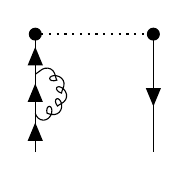
\begin{tikzpicture}[baseline=(a.base)]
		\begin{feynman}
			\node[dot] (a);
			\node[right=\FDWidth of a,dot] (b);
			\vertex[below=\FDHeight of a] (exa);
			\vertex[below=\FDHeight of b] (exb);
			\vertex at ($(exa)!0.33!(a)$) (a1);
			\vertex at ($(exa)!0.66!(a)$) (a2);
			\diagram*{
				(a) --[ghost] (b);
				(exa) --[fermion] (a1) --[fermion] (a2) --[fermion] (a);
				(b) --[fermion] (exb);
				(a1) --[gluon, half right,looseness=2] (a2);
			};
		\end{feynman}
	\end{tikzpicture}
	\hspace{1in}
	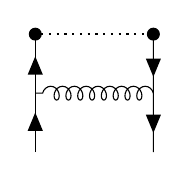
\begin{tikzpicture}[baseline=(a.base)]
		\begin{feynman}
			\node[dot] (a);
			\node[right=\FDWidth of a,dot] (b);
			\vertex[below=\FDHeight of a] (exa);
			\vertex[below=\FDHeight of b] (exb);
			\vertex at ($(exa)!0.5!(a)$) (a1);
			\vertex at ($(exb)!0.5!(b)$) (b1);
			\diagram*{
				(a) --[ghost] (b);
				(exa) --[fermion] (a1) --[fermion] (a);
				(b) --[fermion] (b1) --[fermion] (exb);
				(b1) --[gluon] (a1);
			};
		\end{feynman}
	\end{tikzpicture}
\end{align}

\appendix
\section{Conventions}
The quark field $\psi$ reads
\begin{align}
	\psi(x)=\int \frac{\dd^{3} \vec{k}}{(2 \pi)^{3}} \frac{1}{2 E_{k}}\left[u(k) e^{-i k \cdot x} b_{k}+v(k)e^{ik\cdot x} d_{k}^{\dagger}\right]
\end{align}
and the projection of single particle state is 
\begin{align}
	\ket{p}=b_p^{\dagger}\ket{0}
\end{align}
\begin{align}
	\Bqty{b_{\vb{p}}^r,b_{\vb{q}}^{s\dagger}}=(2\pi)^32E\delta^{(3)}(\vb{p}-\vb{q})\delta^{rs}
\end{align}
The Dirac spinor is normalized to 
\begin{align}
	\bar u^s(p) u(p)=2m\delta^{rs}
\end{align}

\bibliography{../Bib}
\bibliographystyle{apsrev4-1}
\end{document}
